% \documentclass{article}
% \usepackage{beamerarticle}
\documentclass{beamer}
% Beamer theme settings
\usetheme{Madrid}
\usecolortheme{default}
\usepackage{amsmath}

\usepackage{tikz}
% \usepackage{physics}
\usetikzlibrary{calc}
\tikzset{>=latex} % for LaTeX arrow head
\usepackage{xcolor}
\colorlet{veccol}{green!45!black}
\colorlet{myred}{red!90!black}
\colorlet{myblue}{blue!90!black}
\colorlet{mypurple}{blue!50!red!80!black!80}
\tikzstyle{vector}=[->,very thick,veccol]
\usetikzlibrary{arrows.meta}
\tikzstyle{thin arrow}=[dashed,thin,-{Latex[length=4,width=3]}]



\usetikzlibrary{intersections}


% Define commands for vectors
\newcommand{\va}{\mathbf{a}}
\newcommand{\vb}{\mathbf{b}}
\newcommand{\vc}{\mathbf{c}}
\newcommand{\vd}{\mathbf{d}}
\newcommand{\ve}{\mathbf{e}}
\newcommand{\vv}{\mathbf{v}}
\newcommand{\vu}{\mathbf{u}}
\newcommand{\vw}{\mathbf{w}}
\newcommand{\vx}{\mathbf{x}}
\newcommand{\vy}{\mathbf{y}}
\newcommand{\vz}{\mathbf{z}}
\newcommand{\N}{\mathbb{N}}
\newcommand{\Z}{\mathbb{Z}}
\newcommand{\R}{\mathbb{R}}
\newcommand{\Q}{\mathbb{Q}}







% Title page

\title[Lecture 2]{Geometry of Vectors, Matrices}
\author[Aprikyan, Tarkhanyan]{Hayk Aprikyan, Hayk Tarkhanyan}
\institute[ACA]{Armenian Code Academy}
\date{March 21, 2025}
\begin{document}

\begin{frame}
  \titlepage
\end{frame}



% ՆՇՈՒՄ։
% Սկսի նրանից, որ տեսեք, վեկտորների գումարը բլա բլա
% ու վեկտորները ունեն էս էս հատկությունները
% անվանենք վ․ս․
% իսկ այ օրինակ y=4x գծի վրիններն էլ էդ նույնը ունեն, դրանց էլ անվանենք սաբսփեյս 
% ու երևի նորմ բան ասենք, հետո նոր էս



\begin{frame}{Norm}

  What if we want to measure the length of some vector?
\begin{figure}
    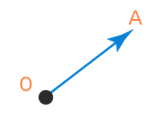
\includegraphics[width=0.25\linewidth]{vector.png}
\end{figure}

\pause 

What we can say, is that 
\[\text{the length of the vector}\]
\[=\]
\[\text{the distance between } O \text{ and } A.\]
  
\end{frame}


\begin{frame}{Norm}
But how to measure distance?

\bigskip 


\pause

\begin{columns}
\begin{column}{0.5\textwidth}
    \begin{center}
     
\includegraphics[width=0.35\textwidth]{chess_1.png}
     \end{center}
    \begin{center}
     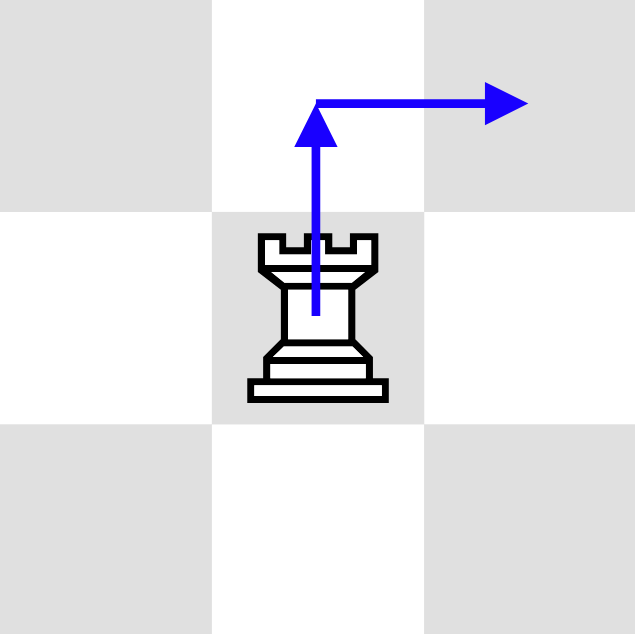
\includegraphics[width=0.35\textwidth]{chess_2.png}
     \end{center}

\end{column}
\begin{column}{0.5\textwidth}  %%<--- here

For a bishop, the distance to its upper-right neighbor is $1$.

\vspace{4em}

While for a rook, it is $2$.

\end{column}
\end{columns}

\pause

\bigskip 
\bigskip 

So there are different ways to measure distance and length.



\end{frame}
\begin{frame}{Norm}

    For a vector $\mathbf{v} = \begin{bmatrix} v_1 \\ v_2 \\ \dots \\ v_n \end{bmatrix}$ in $\mathbb{R}^n$, its \textbf{Euclidean norm} or \textbf{L2 norm} is:
    \[ \|\mathbf{v}\|_2 = \sqrt{v_1^2 +v_2^2+\dots+ v_n^2} \]
    or, equivalently,
    \[ \|\vv\|_2 = \sqrt{\vv \cdot \vv} \]

  \pause

  \begin{example}
    Let $\mathbf{v} = \begin{bmatrix} 3 \\ 4 \end{bmatrix}$. The Euclidean norm of $\mathbf{v}$ is:
    \[ \|\mathbf{v}\|_2 = \sqrt{3^2 + 4^2} = 5 \]
  \end{example}

\pause Euclidean norm is the standard length we use in classic geometry. Sometimes we omit the little "2" and just write $\|\mathbf{v}\|$ instead of $\|\mathbf{v}\|_2$.
\end{frame}

\begin{frame}{Norm}
    For a vector $\mathbf{v} = \begin{bmatrix} v_1 \\ v_2 \\ \dots \\ v_n \end{bmatrix}$ in $\mathbb{R}^n$, its \textbf{Manhattan norm} or \textbf{L1 norm} is:
    \[ \|\mathbf{v}\|_1 = |v_1| + |v_2| + \dots + |v_n| \]

  \pause

 \begin{example}
    Let $\mathbf{v} = \begin{bmatrix} 3 \\ 4 \end{bmatrix}$. The Manhattan norm of $\mathbf{v}$ is:
    \[ \|\mathbf{v}\|_1 = |3| + |4| = 7 \]
  \end{example}



\end{frame}

\begin{frame}
  \frametitle{Norm}

As we have seen, there are different types of norms   (=many different ways to calculate  the length of a vector), and one of them is chosen depending  on the problem.

\pause

\bigskip 


Notice, however, that independently of which one we take, all norms always satisfy the following three properties:
  

\begin{enumerate}
    \item $\|\vv\|\ge 0$, and equals 0 if only if $\vv=\mathbf{0}$,
    \item $\|c\vv\| = |c|\cdot \|\vv\|$,
    \item $\|\vv+\vu\| \le \|\vv\|+\|\vu\|$.
\end{enumerate}

% \begin{figure}
%     \centering
%     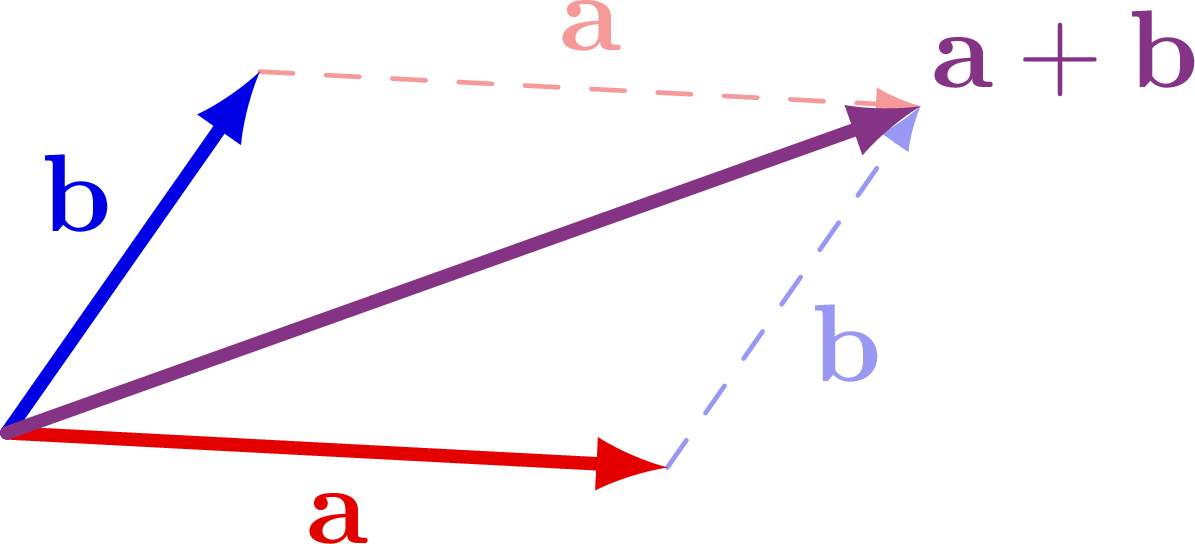
\includegraphics[width=0.4\linewidth]{triangle_ineq.png}
% \end{figure}

\begin{figure}
    \centering
% TWO VECTORS SUM
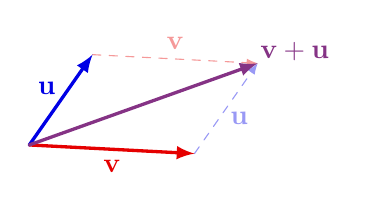
\begin{tikzpicture}[line cap=round]
  \coordinate (O) at (0,0);
  \coordinate (A) at ( -3:2.1);
  \coordinate (B) at ( 55:1.4);
  \coordinate (A+B) at ($(A)+(B)$);
  
  \draw[vector,thin arrow,myred!40] (B) -- (A+B) node[midway,above] {$\vv$};
  \draw[vector,thin arrow,myblue!40] (A) -- (A+B) node[midway,below right=-2] {$\vu$};
  
  \draw[vector,myred] (O) -- (A) node[midway,below] {$\vv$};
  \draw[vector,myblue] (O) -- (B) node[midway,above left=-2] {$\vu$};
  \draw[vector,mypurple] (O) -- (A+B) node[above right=-3] {$\vv+\vu$};
\end{tikzpicture}
\end{figure}


\end{frame}

\begin{frame}{Norm}
    \begin{figure}
        \centering
        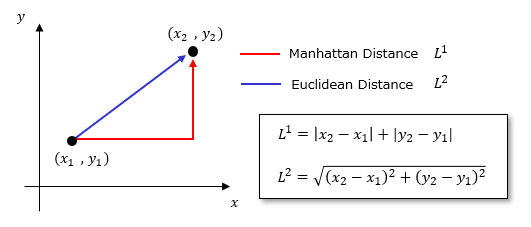
\includegraphics[width=\linewidth]{l1 l2 norms.png}
        
        
    \end{figure}
\end{frame}


% Slide : angles

\begin{frame}
  \frametitle{Angle between vectors}
Geometrically, a vector is an arrow in space, that is, it has both a length and direction. \pause How do we describe a direction in mathematics? \pause By angles!
\bigskip

  \begin{center}
      
\begin{tikzpicture}
  % Define vectors
  \coordinate (O) at (0,0);
  \coordinate (U) at (2,2);
  \coordinate (V) at (4,1);

  % Draw vectors
  \draw[->,thick] (O) -- (U) node[midway, left] {$\mathbf{u}$};
  \draw[->,thick] (O) -- (V) node[midway, below] {$\mathbf{v}$};
\draw[blue] (1, 0.27) arc[start angle=30, end angle=60, radius=1, "$\theta$"];

\end{tikzpicture}
  \end{center}

  \pause \bigskip  Remember the formula from high school geometry: \\$\va \cdot \vb = \|\va\| \|\vb\| \cos\alpha$, where $\alpha$ is the angle between $\va$ and $\vb$.

\end{frame}


% Slide: angles def
\begin{frame}
  \frametitle{Angle between vectors}
\begin{block}{Definition}
    The angle $\theta$ between two vectors $\mathbf{u}$ and $\mathbf{v}$ is the angle $0 \le \theta \le \pi$ for which:
    \[ \cos \theta = \frac{\mathbf{u} \cdot \mathbf{v}}{\|\mathbf{u}\| \cdot \|\mathbf{v}\|} \]
  \end{block}
  \pause

  \begin{example}
    Let $\mathbf{u} = \begin{bmatrix} 3 \\ 4 \end{bmatrix}$ and $\mathbf{v} = \begin{bmatrix} 7\\ 1 \end{bmatrix}$. Find the angle $\theta$ between $\mathbf{u}$ and $\mathbf{v}$.
    \[ \cos \theta = \frac{\mathbf{u} \cdot \mathbf{v}}{\|\mathbf{u}\| \cdot \|\mathbf{v}\|}  = \frac{(3 \cdot 7) + (4 \cdot 1)}{\sqrt{3^2 + 4^2} \cdot \sqrt{7^2 + 1^2}} = \frac{25}{\sqrt{25} \cdot \sqrt{50}} =\frac{1}{\sqrt{2}}\]
    \[ \frac{1}{\sqrt{2}}=\cos{\frac{\pi}{4}} \quad \Rightarrow \quad \theta = \arccos \frac{1}{\sqrt{2}} = \frac{\pi}{4}=45^o \]
  \end{example}

\end{frame}



% Slide : Properties of angles
\begin{frame}{Angle between vectors}
  \begin{block}{Corollary 1}
    For any vectors \( \mathbf{u} \), \( \mathbf{v} \in  \mathbb{R}^n \), 
    \[ \vv \cdot \vu  = \|\vv\| \cdot \|\vu\| \cdot \cos{\theta},\]
    where $\theta$ is the angle between $\vv$ and $\vu$.
  \end{block}
  \pause 
  \begin{block}{Corollary 2}
  The dot product of two vectors equals 0 if and only if they are perpendicular to each other (form a $90^\circ$ angle).
  \end{block}
  
  \pause 
  \begin{block}{Corollary 3}
 Any vector \( \mathbf{v} \in  \mathbb{R}^n \) forms an angle of $0^\circ$ with itself and $180^\circ$ with its negative.
  \end{block}
  
\end{frame}




% Slide 12: Vector space
\begin{frame}{Vector Space}

Finally, we are left to notice two things. Take, for example, 
\begin{itemize}
    \item the set $D=\{0, 1, 2, \dots, 9\}$ of digits, and
    \item the set $P=\{x \in \R : x > 0\}$ of positive numbers.
\end{itemize}

\pause

Notice that,
\begin{itemize}
    \item while the sum of two digits may not be a digit (e.g. $5+7=12$), the sum of two vectors is \textit{always} a vector,
\end{itemize} \pause
and
\begin{itemize}
    \item while the product of a positive number with an arbitrary scalar $c$ may not be positive (e.g. $4 \cdot (-1)=-4$), the product of a vector with a scalar is \textit{always} a vector.
\end{itemize}

\pause

In this case we say that the set of vectors is \textbf{closed under addition and scalar multiplication}, while $D$ or $P$ are not ($P$ is closed under addition only).

\end{frame}

\begin{frame}{Vector Space}
Furthermore, take the line $y=2x$ and choose any  vector on it:
\begin{figure}
    \centering
    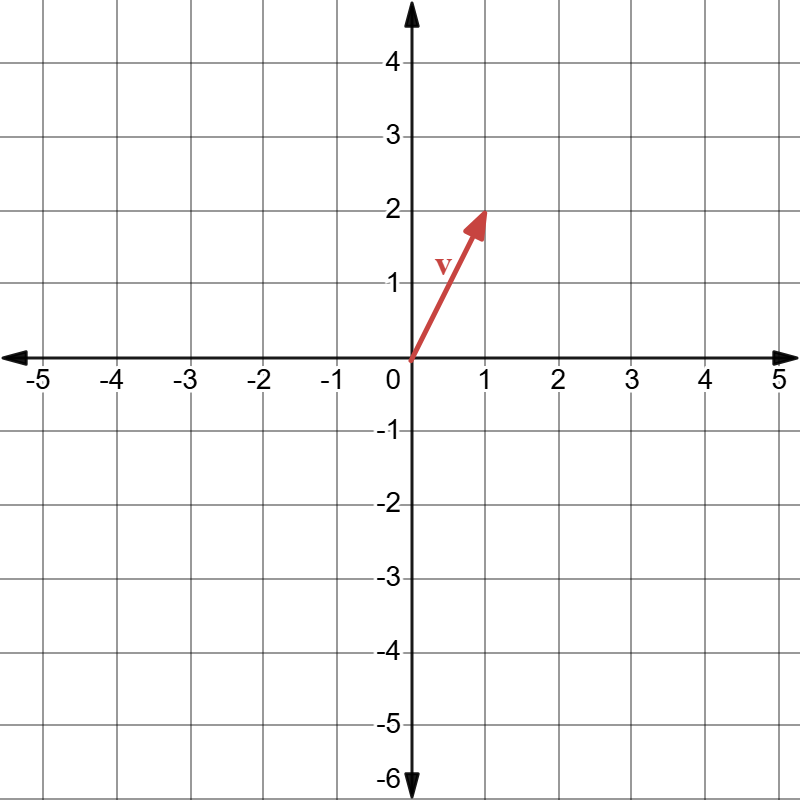
\includegraphics[width=0.5\linewidth]{y=2x 1.png}
\end{figure}

    
\end{frame}


\begin{frame}{Vector Space}
After multiplying it with any number $c$, it will still stay on the line $y=2x$:


\begin{figure}
    \centering
    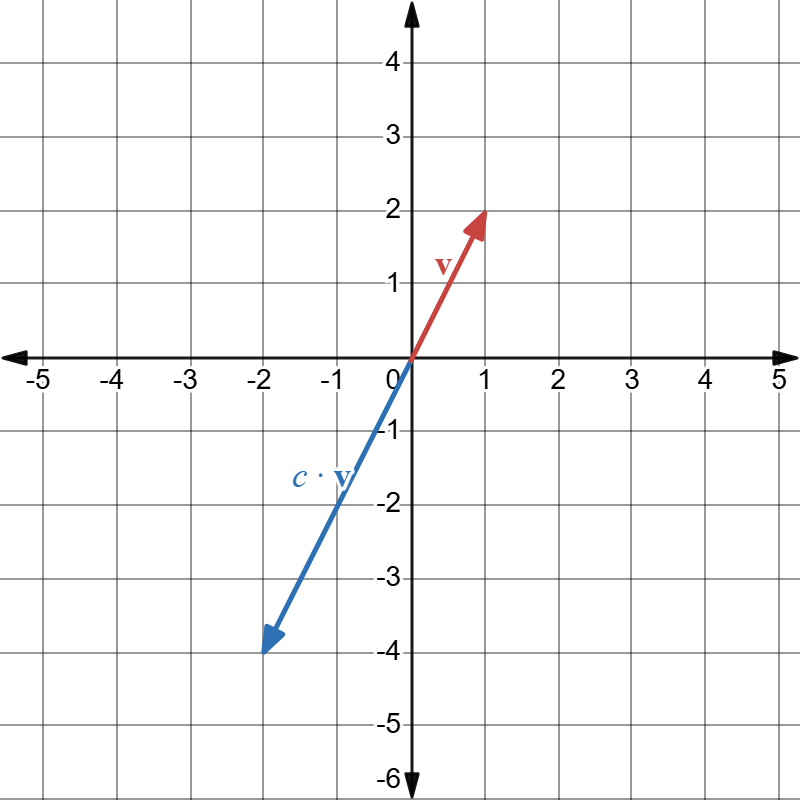
\includegraphics[width=0.5\linewidth]{y=2x 2.png}
\end{figure}
    
\end{frame}





\begin{frame}{Vector Space}
Similarly, if we add two vectors $\vv_1$ and $\vv_2$ which both lie on the line $y=2x$, their sum would again be on the same line.

\pause

\bigskip 

In other words, the line $y=2x$ is \textbf{closed under addition and scalar multiplication}, just like the whole set of vectors $\R^2$. This motivates us to give a special name to the good sets like the line $y=2x$ and $\R^2$.

\pause

\bigskip

We say that $\R^2$ is a \textbf{vector space}, and the set of vectors lying on the line $y=2x$ are a \textbf{vector subspace} of $\R^2$.

\end{frame}

\begin{frame}{Vector Space}
  \begin{block}{Definition}
    A set $V$ is called a \textbf{vector space} if
    \begin{enumerate}
    \item it is closed under addition and scalar multiplication,
      \item \( (\mathbf{u} + \mathbf{v}) + \mathbf{w} = \mathbf{u} + (\mathbf{v} + \mathbf{w}) \)
      \item \( \mathbf{u} + \mathbf{v} = \mathbf{v} + \mathbf{u} \)
      \item There exists a vector \( \mathbf{0} \) such that \( \mathbf{v} + \mathbf{0} = \mathbf{v} \) for all \( \mathbf{v} \in V \)
      \item For every \( \mathbf{v} \in V \), there exists a vector \( -\mathbf{v} \) such that \( \mathbf{v} + (-\mathbf{v}) = \mathbf{0} \)
      \item \( (cd) \cdot \mathbf{v} = c \cdot (d \cdot \mathbf{v}) \)
      \item \( 1 \cdot \mathbf{v} = \mathbf{v} \)
      \item \( c \cdot (\mathbf{u} + \mathbf{v}) = c \cdot \mathbf{u} + c \cdot \mathbf{v} \)
      \item \( (c + d) \cdot \mathbf{v} = c \cdot \mathbf{v} + d \cdot \mathbf{v} \)
    \end{enumerate}
  \end{block}
    
  No need to memorize the properties--just the natural laws of addition and scalar multiplication. 
\end{frame}

% % Slide 1: subset
% \begin{frame}{Subspaces}
% Let $A$ be some set.
%     \begin{block}{Definition}
%     The set $B$ is called a \textbf{subset} of $A$, if all of its elements are also elements of $A$. %\pause $A$ is called the \textbf{superset}.
%   \end{block}

%   \pause In other words, a subset is another set which is a \textit{part} of the "parent set".

%   \pause We denote "$B$ is a subset of $A$" by $B\subset A$ or $B\subseteq A$.

%   \begin{example}
%     If $A = \{1, 2, 3, 4\}$, $B = \{2, 4\}$ and $C = \{2, 5\}$, then $B \subset A$ but $C \not\subset A$.
%   \end{example}

%   \pause

%   \begin{block}{Properties}
%       \begin{itemize}
%           \item Every set is its own subset: $A\subset A$,
%           \item Empty set is a subset for any set: $\emptyset\subset A$,
%           \item If both $A\subset B$ and $B\subset A$, then $A=B$.
%       \end{itemize}
%       \end{block}

% \end{frame}

% % % Slide 2: subspace
% % \begin{frame}{Subspaces}
% %   \begin{itemize}[<+->]
% %     \item Oftentimes we are interested in checking whether a given set, together with given operations of addition ($+$) and multiplication by scalar ($\cdot$), is a vector space.
    
% %     \item We need to show that the set:
% %     \begin{itemize}
% %         \item[A: ] is closed under \textit{addition} and \textit{multiplication by scalar}:\\(for all $\vx, \vy$ elements and $c\in\R$ scalars, both $\vx+\vy$ and $c\vx$ belong to the set)
% %         \item[B: ] satisfies the conditions 1-8 of a vector space.
% %     \end{itemize}
    
% %     \item Suppose we have already shown that our set is a subset of some vector space.

% %     For example, $A = \bigg\{ \begin{bmatrix} a \\ 0 \end{bmatrix} \mid \text{ for all numbers }a\in\R\bigg\} \subset \R^2.$

% %     \item How can we check if $A$ is a vector space, knowing that $\R^2$ is a vector space?
% %   \end{itemize}
% % \end{frame}

% Slide 3: Definition
\begin{frame}{Vector Space}
  \begin{block}{Definition}
   A subset $U$ of a vector space $V$ is called a \textbf{subspace} of $V$
 if $U$ itself is a vector space.
\end{block}

\pause How to check if a subset $U$ of $V$ is a sub\textit{space}? Just make sure that it is closed under addition and scalar multiplication!

\pause  \begin{block}{Theorem}
  Assume $V$ is a vector space, and $U$ is  a subset of $V$. Then $U$ is a subspace of $V$ if and only if 
      \begin{itemize}
          \item[1.] $\vx+\vy \in U$, for all $\vx,\vy\in U$,
          \item[2.] $c\vx \in U$, for all $\vx\in U$ and $c\in\R$.
      \end{itemize}
\end{block}

\pause

\begin{itemize}
    \item So $\R^1$, $\R^2$, $\R^3$, $\dots$ are all vector spaces. 
    \item The set of all vectors that lie on the same line (e.g. $y=kx$) form a  subspace (on the condition that  the line also contains the \textbf{0} vector).
\end{itemize}

  \end{frame}

% % Slide 4: Examples
% \begin{frame}{Subspaces}
%  \begin{example}
%      In our example, $A = \bigg\{ \begin{bmatrix} a \\ 0 \end{bmatrix} \mid \text{ for all numbers }a\in\R\bigg\} \subset \R^2$, and we already know that $\R^2$ is a vector space.
%      \pause
%      \begin{itemize}[<+->]
%          \item \[ \begin{bmatrix} a \\ 0 \end{bmatrix}+\begin{bmatrix} b \\ 0 \end{bmatrix} =\begin{bmatrix} a +b\\ 0 \end{bmatrix}\in A \]
         
%          \item \[ c \cdot \begin{bmatrix} a \\ 0 \end{bmatrix}=\begin{bmatrix} ca \\ 0 \end{bmatrix}\in A \]
%      \end{itemize}

%      \pause      Therefore, $A$ is a subspace of $\R^2$.%, and a vector space.
%  \end{example}
% \end{frame}




% matrices
\begin{frame}{Matrices}
\begin{block}{Definition}
An \(m \times n\) tuple $A$ of elements \(a_{ij}\) ($i = 1, \ldots, m$ and $j = 1, \ldots, n$), is called a real-valued \((m, n)\) \textbf{matrix}:

\[
A =
\begin{bmatrix}
    a_{11} & a_{12} & \ldots & a_{1n} \\
    a_{21} & a_{22} & \ldots & a_{2n} \\
    \vdots & \vdots & \ddots & \vdots \\
    a_{m1} & a_{m2} & \ldots & a_{mn}
\end{bmatrix},
\qquad a_{ij} \in \mathbb{R}.
\]
The set of all real-valued $(m,n)$ matrices is denoted by $\R^{m\times n}$. 
\end{block} 

  \begin{example}
    \[
      A = \begin{bmatrix}
        1 & 2 & 3 \\
        4 & 5 & 6 \\
      \end{bmatrix} \in \R^{2\times 3}
      \qquad
      B = \begin{bmatrix}
        -2 & 0 \\
        1 & 3 \\
      \end{bmatrix} \in \R^{2\times 2}
    \]
  \end{example}
\pause Note that the first number in $(m,n)$ \alert{always} shows rows, second: columns.
\end{frame}




\begin{frame}
  \frametitle{Matrix Addition}
The vectors are practically 1-column matrices: $\R^n = \R^{n\times 1}$. Similar to vectors, we define the following operations with the matrices:
  \pause

  \begin{block}{Definition}
    The sum of two matrices \(A\) and \(B\), denoted as \(A + B\), is obtained by adding corresponding elements. If \(A\) is of size \(m \times n\) and \(B\) is of the same size, then \(A + B\) is also of size \(m \times n\).
       \[
      A = \begin{bmatrix}
        a_{11} & a_{12} & \ldots & a_{1n} \\
        a_{21} & a_{22} & \ldots & a_{2n} \\
        \vdots & \vdots & \ddots & \vdots \\
        a_{m1} & a_{m2} & \ldots & a_{mn} \\
      \end{bmatrix}
      \quad
      B = \begin{bmatrix}
        b_{11} & b_{12} & \ldots & b_{1n} \\
        b_{21} & b_{22} & \ldots & b_{2n} \\
        \vdots & \vdots & \ddots & \vdots \\
        b_{m1} & b_{m2} & \ldots & b_{mn} \\
      \end{bmatrix}
    \]

    \[
      A + B = \begin{bmatrix}
        a_{11} + b_{11} & a_{12} + b_{12} & \ldots & a_{1n} + b_{1n} \\
        a_{21} + b_{21} & a_{22} + b_{22} & \ldots & a_{2n} + b_{2n} \\
        \ldots & \ldots & \ldots & \ldots \\
        a_{m1} + b_{m1} & a_{m2} + b_{m2} & \ldots & a_{mn} + b_{mn} \\
      \end{bmatrix}
    \]
  \end{block}


\end{frame}

\begin{frame}
  \frametitle{Matrix Addition}
  \begin{example}
    \[
      A = \begin{bmatrix}
        1 & 2 \\
        3 & 4 \\
      \end{bmatrix}
      \quad
      B = \begin{bmatrix}
        -2 & 0 \\
        1 & 3 \\
      \end{bmatrix}
    \]
    \[
      A + B = \begin{bmatrix}
        -1 & 2 \\
        4 & 7 \\
      \end{bmatrix}
    \]
  \end{example}

  \pause

  \begin{block}{Remark}
    Matrix addition is only defined for matrices of the same size.
  \end{block}
\end{frame}


\begin{frame}
  \frametitle{Scalar Multiplication of a Matrix}

  \begin{block}{Definition}
    The product of a scalar \(c\) and a matrix \(A\), denoted as \(cA\), is obtained by multiplying each element of the matrix by the scalar.
  \[
      c \cdot A = c \cdot \begin{bmatrix}
        a_{11} & a_{12} & \ldots & a_{1n} \\
        a_{21} & a_{22} & \ldots & a_{2n} \\
        \vdots & \vdots & \ddots & \vdots \\
        a_{m1} & a_{m2} & \ldots & a_{mn} \\
      \end{bmatrix}
    \]
    
    \[
      = \begin{bmatrix}
        c \cdot a_{11} & c \cdot a_{12} & \ldots & c \cdot a_{1n} \\
        c \cdot a_{21} & c \cdot a_{22} & \ldots & c \cdot a_{2n} \\
        \vdots & \vdots & \ddots & \vdots \\
        c \cdot a_{m1} & c \cdot a_{m2} & \ldots & c \cdot a_{mn} \\
      \end{bmatrix}
    \]
  \end{block}
  \pause

    Scalar multiplication can be performed for any scalar \(c\) and any matrix \(A\).

\end{frame}



\begin{frame}
  \frametitle{Negative of a Matrix}

  \begin{block}{Definition}
    The negative of a matrix \(A\), denoted as \(-A\), is obtained by changing the sign of each element in the matrix.

    \[
      -A = -\begin{bmatrix}
        a_{11} & a_{12} & \ldots & a_{1n} \\
        a_{21} & a_{22} & \ldots & a_{2n} \\
        \ldots & \ldots & \ldots & \ldots \\
        a_{m1} & a_{m2} & \ldots & a_{mn} \\
      \end{bmatrix}
    \]
    
    \[
      = \begin{bmatrix}
        -a_{11} & -a_{12} & \ldots & -a_{1n} \\
        -a_{21} & -a_{22} & \ldots & -a_{2n} \\
         \ldots & \ldots & \ldots & \ldots \\
        -a_{m1} & -a_{m2} & \ldots & -a_{mn} \\
      \end{bmatrix}
    \]
  \end{block}

  \pause

  \begin{block}{Remark}
    The negative of a matrix equals $(-1)$ times the matrix.
  \end{block}

\end{frame}

\begin{frame}
  \frametitle{Matrix Subtraction}

  \begin{block}{Definition}
    The difference of two matrices \(A\) and \(B\), denoted as \(A - B\), is obtained by subtracting corresponding elements, or by adding $A$ and $-B$. If \(A\) and \(B\) are both of size \(m \times n\), then \(A - B\) is also of size \(m \times n\).
    \[
      A = \begin{bmatrix}
        a_{11} & a_{12} & \ldots & a_{1n} \\
        a_{21} & a_{22} & \ldots & a_{2n} \\
         \ldots & \ldots & \ldots & \ldots  \\
        a_{m1} & a_{m2} & \ldots & a_{mn} \\
      \end{bmatrix}
      \quad
      B = \begin{bmatrix}
        b_{11} & b_{12} & \ldots & b_{1n} \\
        b_{21} & b_{22} & \ldots & b_{2n} \\
        \ldots & \ldots & \ldots & \ldots  \\
        b_{m1} & b_{m2} & \ldots & b_{mn} \\
      \end{bmatrix}
    \]

    \[
      A - B = \begin{bmatrix}
        a_{11} - b_{11} & a_{12} - b_{12} & \ldots & a_{1n} - b_{1n} \\
        a_{21} - b_{21} & a_{22} - b_{22} & \ldots & a_{2n} - b_{2n} \\
         \ldots & \ldots & \ldots & \ldots \\
        a_{m1} - b_{m1} & a_{m2} - b_{m2} & \ldots & a_{mn} - b_{mn} \\
      \end{bmatrix}
    \]
  \end{block}

  \pause

    Matrix subtraction is only defined for matrices of the same size.

\end{frame}

\begin{frame}
  \frametitle{Zero Matrix}

  \begin{block}{Definition}
    The \textbf{zero matrix}, denoted as \(O\) or \(O_{m \times n}\), is a matrix where all elements are zero.
  \end{block}

  \pause

  \begin{example}
    \[
      O_{2 \times 3} = \begin{bmatrix}
        0 & 0 & 0 \\
        0 & 0 & 0 \\
      \end{bmatrix}
      \quad
      O_{3 \times 2} = \begin{bmatrix}
        0 & 0 \\
        0 & 0 \\
        0 & 0 \\
      \end{bmatrix}
    \]
  \end{example}

  \pause

  \begin{block}{Remark}
    \(A + O=O+A= A\) for any matrix \(A\).
  \end{block}

\end{frame}


\begin{frame}
  \frametitle{Transpose of a Matrix}

  \begin{block}{Definition}
    The \textbf{transpose} of a matrix \(A\), denoted as \(A^T\), is obtained by swapping its rows and columns.
    \[A = \begin{bmatrix}
        a_{11} & a_{12} & \ldots & a_{1n} \\
        a_{21} & a_{22} & \ldots & a_{2n} \\
         \ldots & \ldots & \ldots & \ldots  \\
        a_{m1} & a_{m2} & \ldots & a_{mn} \\
      \end{bmatrix}\qquad A^T = \begin{bmatrix}
        a_{11} & a_{21} & \ldots & a_{n1} \\
        a_{12} & a_{22} & \ldots & a_{n2} \\
         \ldots & \ldots & \ldots & \ldots  \\
        a_{1m} & a_{2m} & \ldots & a_{nm} \\
      \end{bmatrix}\]
  \end{block}

  \pause

  \begin{example}
    \[
      A = \begin{bmatrix}
        7&4&2\\0&1&-3
      \end{bmatrix}\qquad
      A^T = \begin{bmatrix}
        7 & 0 \\
        4 & 1 \\
        2 & -3
      \end{bmatrix}
    \]
  \end{example}

  \pause

  \begin{block}{Remark}
    The transpose of an $(m,n)$ matrix is an $(n,m)$ matrix.
  \end{block}

\end{frame}


\begin{frame}{Matrices}
    Matrices can be added together and multiplied by numbers, and these operations share the same "good" properties (e.g. $A+B=B+A$) with vectors. \pause

    \bigskip 
    In that sense, it is not difficult to prove that:
\bigskip
    \begin{block}{Theorem}
    For each $m,n\in\N$ the set of real-valued matrices $\R^{m\times n}$ forms a vector space.

    \end{block}
\end{frame}


% Slide 1: matrix vector
\begin{frame}{Matrix-Vector Multiplication}

  \begin{block}{Definition}
    Let \(A\) be an \(m \times n\) matrix and \(\mathbf{v}\) be a column vector of size \(n \times 1\). The product \(A\mathbf{v}\) is a column vector of size \(m \times 1\) obtained by multiplying each row of \(A\) by the corresponding element of \(\mathbf{v}\) and summing the results.

    \[
      A = \begin{bmatrix}
        a_{11} & a_{12} & \ldots & a_{1n} \\
        a_{21} & a_{22} & \ldots & a_{2n} \\
        \vdots & \vdots & \ddots & \vdots \\
        a_{m1} & a_{m2} & \ldots & a_{mn} \\
      \end{bmatrix}
      \quad
      \mathbf{v} = \begin{bmatrix}
        v_1 \\
        v_2 \\
        \vdots \\
        v_n \\
      \end{bmatrix}
    \]

    \[
      A\mathbf{v} = \begin{bmatrix}
        a_{11}v_1 + a_{12}v_2 + \ldots + a_{1n}v_n \\
        a_{21}v_1 + a_{22}v_2 + \ldots + a_{2n}v_n \\
        \vdots \\
        a_{m1}v_1 + a_{m2}v_2 + \ldots + a_{mn}v_n \\
      \end{bmatrix}
    \]
  \end{block}
    

  % \pause

  % \begin{block}{Remark}
  %   Matrix-vector multiplication transforms a vector based on the linear transformation represented by the matrix.
  % \end{block}

\end{frame}


% Slide 1: matrix vector
\begin{frame}{Matrix-Vector Multiplication}

  Or, in other words, if we denote the rows of $A$ by \(\mathbf{A}_1, \mathbf{A}_2, \ldots, \mathbf{A}_m\), the product \(A\mathbf{v}\) will be a column vector of size \(m \times 1\) obtained by taking the dot product of each row of \(A\) with the vector \(\mathbf{v}\):
    \[
      A = \begin{bmatrix}
        \dots& \mathbf{A}_1 & \ldots \\
        \dots& \mathbf{A}_2 & \ldots \\
         & \vdots &  \\
        \dots& \mathbf{A}_m & \ldots \\
      \end{bmatrix}
      \qquad
      \mathbf{v} = \begin{bmatrix}
        v_1 \\
        v_2 \\
        \vdots \\
        v_n \\
      \end{bmatrix}
    \]

    \[
      A\mathbf{v} = \begin{bmatrix}
        a_{11}v_1 + a_{12}v_2 + \ldots + a_{1n}v_n \\
        a_{21}v_1 + a_{22}v_2 + \ldots + a_{2n}v_n \\
        \vdots \\
        a_{m1}v_1 + a_{m2}v_2 + \ldots + a_{mn}v_n \\
      \end{bmatrix}= \begin{bmatrix}
        \mathbf{A}_1 \cdot \mathbf{v} \\
        \mathbf{A}_2 \cdot \mathbf{v} \\
        \vdots \\
        \mathbf{A}_m \cdot \mathbf{v} \\
      \end{bmatrix} 
    \]
    

  % \pause

  % \begin{block}{Remark}
  %   Matrix-vector multiplication transforms a vector based on the linear transformation represented by the matrix.
  % \end{block}

\end{frame}


% Slide 1: matrix vector
\begin{frame}{Matrix-Vector Multiplication}
  \begin{center}
    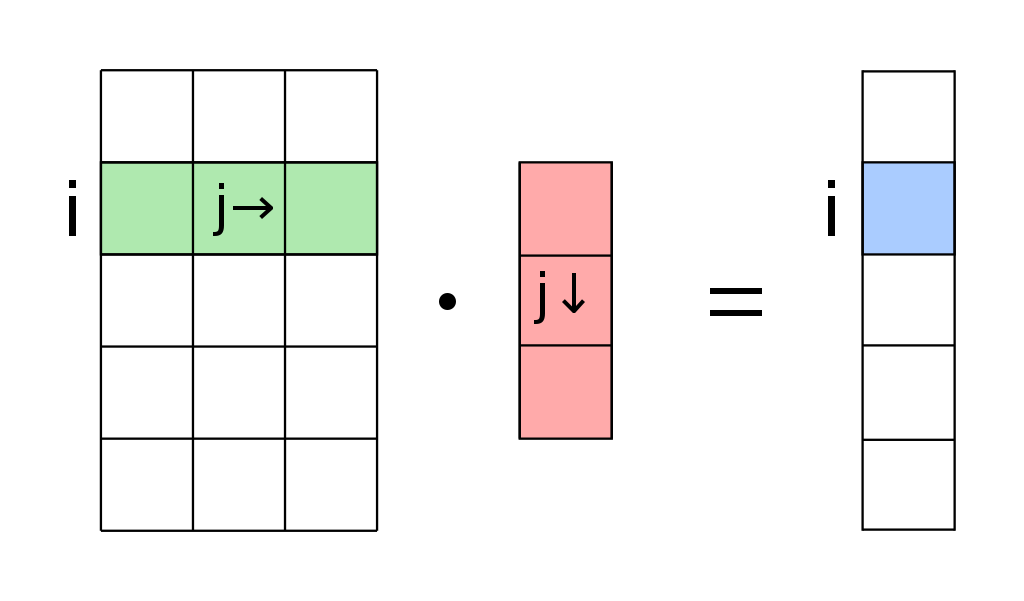
\includegraphics[width=\textwidth, height=\textheight, keepaspectratio]{mvm.png}
  \end{center}
  \end{frame}

% Slide 1: matrix vector
\begin{frame}{Matrix-Vector Multiplication}
  \begin{example}
    \[
      A = \begin{bmatrix}
        1 & 2 & 3 \\
        4 & 5 & 6 \\
      \end{bmatrix}
      \quad
      \mathbf{v} = \begin{bmatrix}
        2 \\
        -1 \\
        3 \\
      \end{bmatrix}
    \]

    \[
      A\mathbf{v} = \begin{bmatrix}
        1 \cdot 2 + 2 \cdot (-1) + 3 \cdot 3 \\
        4 \cdot 2 + 5 \cdot (-1) + 6 \cdot 3 \\
      \end{bmatrix}
      = \begin{bmatrix}
        9 \\
        21 \\
      \end{bmatrix}
    \]
  \end{example}

  \pause

  \begin{example}
    \[
      A = \begin{bmatrix}
        -2 & 1 \\
        0 & 3 \\
        1 & -1 \\
      \end{bmatrix}
      \quad
      \mathbf{v} = \begin{bmatrix}
        4 \\
        2 \\
      \end{bmatrix}
    \]

    \[
      A\mathbf{v} = \begin{bmatrix}
        (-2) \cdot 4 + 1 \cdot 2 \\
        0 \cdot 4 + 3 \cdot 2 \\
        1 \cdot 4 + (-1) \cdot 2 \\
      \end{bmatrix}
      = \begin{bmatrix}
        -6 \\
        6 \\
        2 \\
      \end{bmatrix}
    \]
  \end{example}
  % \pause

  % \begin{block}{Remark}
  %   Matrix-vector multiplication transforms a vector based on the linear transformation represented by the matrix.
  % \end{block}

\end{frame}


% Slide 1: matrix vector
\begin{frame}{Matrix-Vector Multiplication}
    Matrix-vector multiplication shares properties with scalar multiplication and addition of vectors.

 \begin{itemize}
       \item \textbf{Distributive Property:}

    For a matrix \(A\) and vectors \(\mathbf{v}\) and \(\mathbf{w}\) of appropriate sizes:
    \[
      A(\mathbf{v} + \mathbf{w}) = A\mathbf{v} + A\mathbf{w}
    \]
\item \textbf{Scalar Multiplication:}

    For a matrix \(A\) and a scalar \(c\):
    \[
      A(c\mathbf{v}) = c(A\mathbf{v})
    \]
  \end{itemize}
\pause
    Note that we can only multiply a matrix by a vector if the number of columns of the matrix equals the length of the vector.

\end{frame}




% slide 6: definite
\begin{frame}{Geometric Interpretation }

Why do we define the matrix-vector multiplication this way? Turns out, it has a beautiful geometrical interpretation. \pause 

\bigskip

Think this way: when you multiply, say, a $2\times 2$ matrix $A$ by a vector $\vv\in\R^2$, what you get is another vector $\vu=A\vv\in\R^2$. We call this $\vu$ the \textbf{transformed version} of $\vv$ (and we say that $A$ is a linear transformation).

\begin{figure}
    \centering
    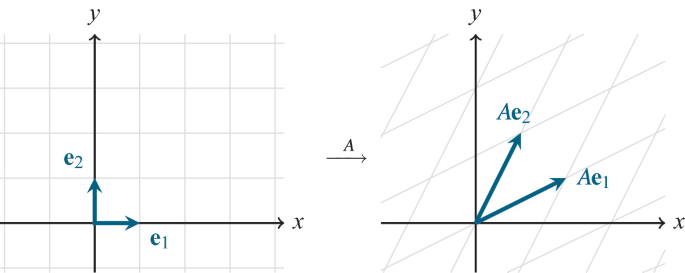
\includegraphics[width=0.75\linewidth]{viz ex.png}
    
    
\end{figure}

\end{frame}


% slide 6: definite
\begin{frame}{Geometric Interpretation }

As we will see later, the resulting "transformed version" $\vu$ is just the same old $\vv$ except it is \textbf{rotated} and \textbf{scaled} to become longer or shorter (and possibly, flipped).

\pause 

\bigskip

In this sense, all  matrices are either just rotating vectors by some degree, or flipping them horizontally/vertically, or scale them, or do all three.

\smallskip 

The key thing is: whatever a matrix "does" to one vector, it does the same to all other vectors too (when being multiplied with them).

\bigskip
\bigskip


{\small
\textcolor{blue}{Check different matrices yourself:\\ - \url{visualize-it.github.io/linear_transformations/simulation.html} 
\\ - \url{www.shad.io/MatVis}
}}

\bigskip

We will learn more about this later--now back to matrices$\sim$

    
\end{frame}





% Slide 2: matrix mult

\begin{frame}
  \frametitle{Matrix Multiplication}

  \begin{block}{Definition}
    Let \(A\) be an \(m \times n\) matrix, and let \(B\) be an \(n \times k\) matrix. The product \(C = AB\) is an \(m \times k\) matrix, where each element \(c_{ij}\) is obtained by taking the dot product of the \(i\)-th row of \(A\) and the \(j\)-th column of \(B\):

\[
      A = \begin{bmatrix}
        a_{11} & a_{12} & \ldots & a_{1n} \\
        a_{21} & a_{22} & \ldots & a_{2n} \\
        \dots & \dots & \dots & \dots \\        a_{m1} & a_{m2} & \ldots & a_{mn} \\
      \end{bmatrix}
      \qquad
      B = \begin{bmatrix}
        b_{11} & b_{12} & \ldots & b_{1k} \\
        b_{21} & b_{22} & \ldots & b_{2k} \\
        \dots & \dots & \dots & \dots \\        b_{n1} & b_{n2} & \ldots & b_{nk} \\
      \end{bmatrix}
    \]

    \[
      C = AB = \begin{bmatrix}
        c_{11} & c_{12} & \ldots & c_{1k} \\
        c_{21} & c_{22} & \ldots & c_{2k} \\
        \dots & \dots & \dots & \dots \\
        c_{m1} & c_{m2} & \ldots & c_{mk} \\
      \end{bmatrix}
    \]

    \[
      \text{where }c_{ij} = a_{i1}b_{1j} + a_{i2}b_{2j} + \ldots + a_{in}b_{nj}= \sum_{p=1}^{n} a_{ip}b_{pj}
    \]
    
  \end{block}

\end{frame}




% Slide 2: matrix mult

\begin{frame}
  \frametitle{Matrix Multiplication}
  \begin{center}
    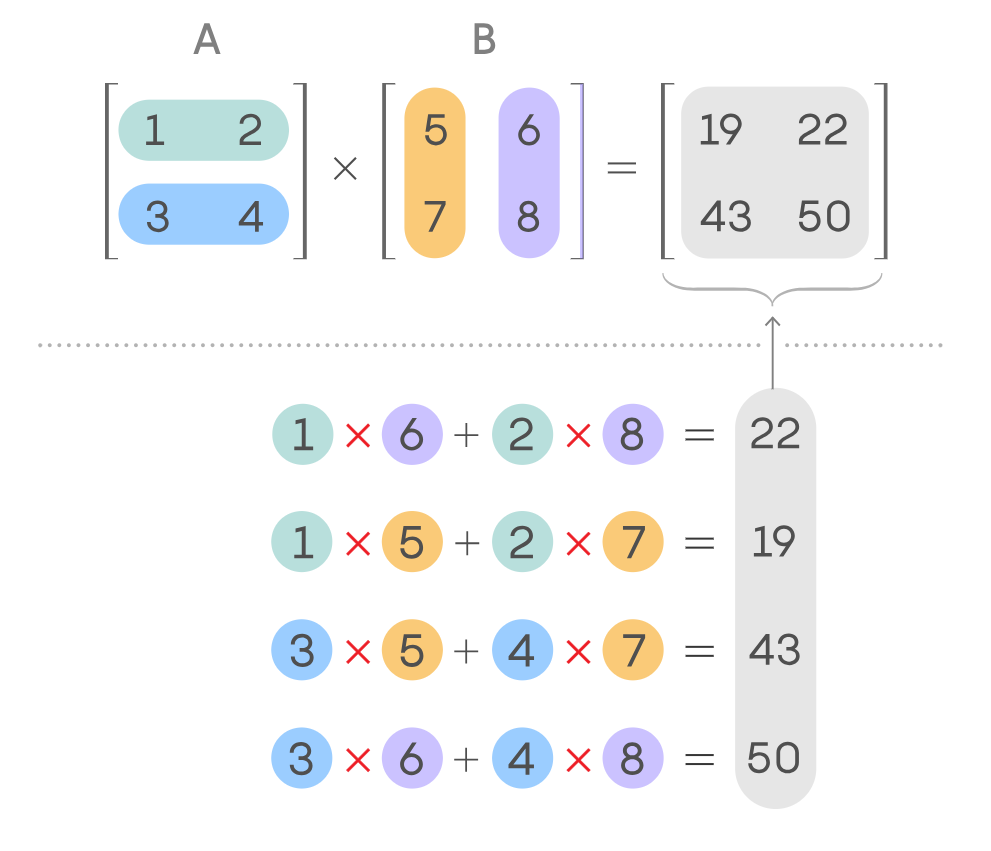
\includegraphics[height=0.9\textheight, keepaspectratio]{mmm.png}
  \end{center}
\end{frame}


% Slide 1: matrix vector
\begin{frame}{Matrix Multiplication}
    Matrix multiplication shares properties with scalar multiplication and addition of vectors, as well as matrix-vector multiplication.
\begin{itemize}
    \item \textbf{Distributive Property:}

    For matrices \(A\), \(B\), and \(C\) of appropriate sizes:
    \[
      A(B + C) = AB + AC \quad \text{and} \quad (A + B)C = AC + BC
    \]

  \item \textbf{Associativity Property:}
  
    For matrices \(A\), \(B\), and \(C\) of appropriate sizes:
    \[
      A(BC) = (AB)C
    \]
  \item \textbf{Scalar Multiplication:}
  
    For matrices \(A\), \(B\) of appropriate sizes and a scalar \(c\):
    \[
      A(cB) = c(AB)=(cA)B
    \]
  \end{itemize}
\pause
    Note that we can only multiply two matrices if the number of columns of the first matrix equals the number of rows of the second matrix: $(m\times n)$ with $(n\times k)$.

\end{frame}



% Slide 3: matrix mult
\begin{frame}{Matrix Multiplication}

  \begin{example}
    Let
    \[
      C = \begin{bmatrix}
        -1 & 0 \\
        2 & -3 \\
        4 & 1 \\
      \end{bmatrix}\in \R^{3 \times 2}
      \qquad
      D = \begin{bmatrix}
        5 & -2 & 1 \\
        3 & 0 & 7 \\
      \end{bmatrix}\in \R^{2 \times 3}
    \]

    \[
      CD = \begin{bmatrix}
        -1 \cdot 5 + 0 \cdot 3 & -1 \cdot (-2) + 0 \cdot 0 & -1 \cdot 1 + 0 \cdot 7 \\
        2 \cdot 5 + (-3) \cdot 3 & 2 \cdot (-2) + (-3) \cdot 0 & 2 \cdot 1 + (-3) \cdot 7 \\
        4 \cdot 5 + 1 \cdot 3 & 4 \cdot (-2) + 1 \cdot 0 & 4 \cdot 1 + 1 \cdot 7 \\
      \end{bmatrix}
     \]\[ = \begin{bmatrix}
        -5 & 2 & -1 \\
        1 & -4 & -19 \\
        23 & -8 & 11 \\
      \end{bmatrix}\in\R^{3 \times 3}
    \]
  \end{example}

\end{frame}




\end{document}
